% Betrag des Frequenzganges U2/U1 in halblogarithmischer Darstellung
% R = 150 Ohm, L = 20 mH, C = 1 µF
% wo= 1/sqrt(L*C)= 7071.068 s^-1
% A(100)=1.000
% A(1000)=1.009
% A(2000)=1.033
% A(3500)=1.087
% A(7071)=0.943
% A(10000)=0.555
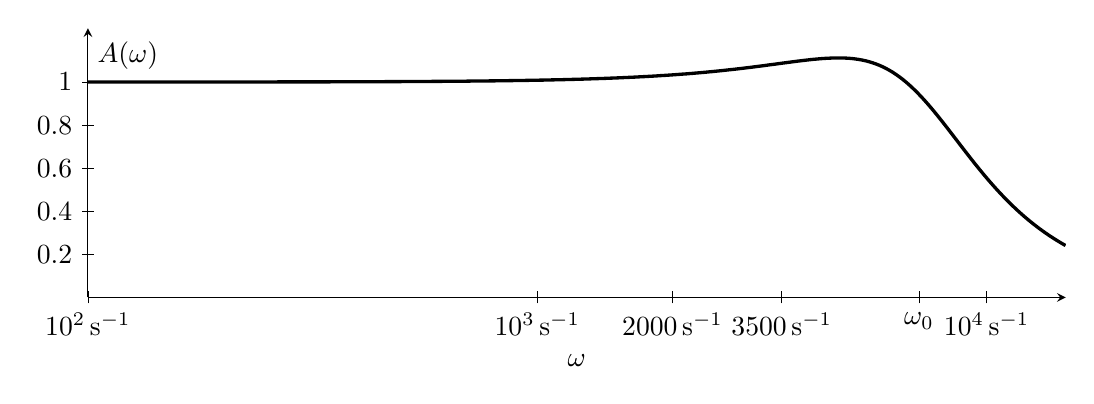
\begin{tikzpicture}[x=1cm,y=1cm]
    \begin{axis}[
        xmode=log,
        ymode=linear,
        xmin=1e2, xmax=15e3,
        ymin=0, ymax=1.25,
        xlabel={$\omega$},
        ylabel style={rotate=-90, at={(axis description cs:0,0.9)}, anchor=west},
        ylabel={$A(\omega)$},
        axis x line= bottom,
        axis y line= left,
        xtick={100,1000, 2000, 3500, 7071, 10000}, % Vorgabe aus Aufgabe
        xticklabels={$10^2\, \mathrm{s}^{-1}$, $10^3 \, \mathrm{s}^{-1}$, $2000 \, \mathrm{s}^{-1}$, $3500 \, \mathrm{s}^{-1}$, $ \omega_0 $, $10^4 \, \mathrm{s}^{-1}$}, 
        ytick={0.2, 0.4, 0.6, 0.8, 1},
        grid=none,
        width=14cm,
        height=5cm,
        tick style={color=black},
        samples=300,
    ]
        %Spannungen
        \addplot[color=black, very thick, domain=100:15000] {1 / (sqrt( (1 - x^2 * 20e-3 * 1e-6)^2 + (x * 150 * 1e-6)^2 ))};
        
    \end{axis}
\end{tikzpicture}